\chapter{Technologie, algorytmy i narzędzia (Piotr Chojnowski)}
\label{chap:algs}

Dzięki dużej popularności urządzeń VR powstało również wiele różnych narzędzi wytwarzania takich aplikacji. W tym rozdziale zostały omówione najbardziej popularne z nich, oraz które z nich wybraliśmy.

\section{Unreal Engine}
Dwa najbardziej znane i używane środowiska w wytwarzaniu aplikacji VR to aktualnie Unreal Engine oraz Unity, więc postanowiliśmy wybrać jeden z nich jako nasze środowisko. Jako że system CAVE, który jest docelową platformą omawianej aplikacji, działa na klastrze, zdecydowaliśmy się ostatecznie na użycie Unreal Engine 5. Doszliśmy do tego wniosku, ponieważ dla środowiska UE5 została stworzona wtyczka nDisplay, która pozwala na automatyczną obsługę takiego klastra. Unreal Engine jest silnikiem stworzonym przez przedsiębiorstwo Epic Games przeznaczonym głównie do tworzenia gier 3D.

\section{ART Flystick}
ART Flystick to bezprzewodowy kontroler opracowany przez firmę Advanced Realtime Tracking. Służy do interakcji w środowiskach VR, AR oraz w systemach śledzenia ruchu, szczególnie w środowiskach naukowych, inżynierskich i medycznych. Jest to kontroler, którego domyślnie używa docelowy system CAVE, więc właśnie pod niego tworzymy naszą aplikację.
\newline
\begin{figure}[h!]
    \centering
    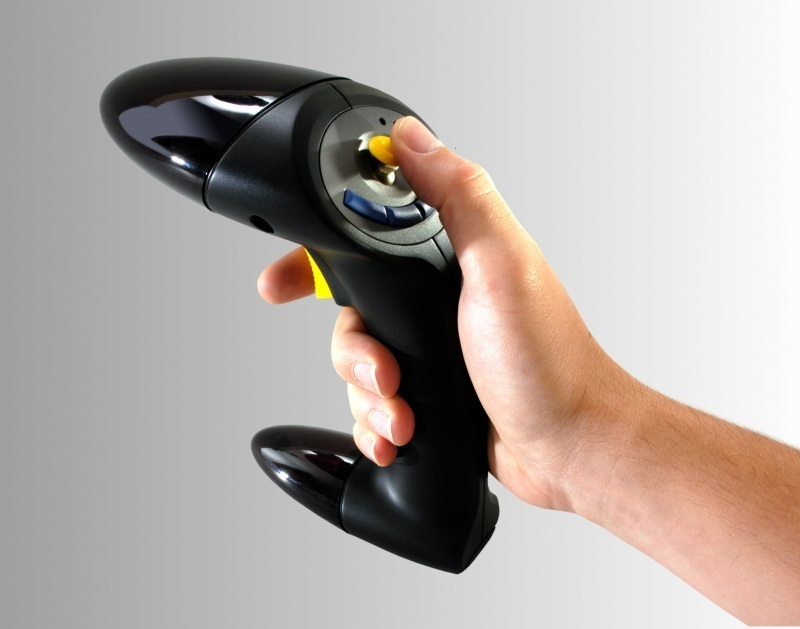
\includegraphics[width=0.6\textwidth]{images/ART Flystick2 small.jpg}
    \caption{Kontroler ART Flystick2 \cite{flystick_img}}
    \label{img:flystick}
\end{figure}

\section{Algorytmy}
W naszych zagadkach użyliśmy kilku gotowych algorytmów z ewentualnymi modyfikacjami. Zostały one przedstawione poniżej.

\subsection{Finite Element Method for Beam and Truss Structures}

Finite Element Method for Beam and Truss Structures jest algorytmem, którego użyliśmy do implementacji zagadki z mechaniki, aby zasymulować łamanie się belek pod odpowiednim ciężarem. Jest to algorytm bazujący na implementacji teorii belki Eulera-Bernoulliego w C++ oraz używający Python 3.7 z bibliotekami matplotlib, PyQt5 i PyQt5-tools do wizualizacji i interfejsu. \cite{FEMBTS_git} Dzięki użyciu C++ przez autora, implementacja algorytmu w środowisku UE5 nie była skomplikowana i wystarczyło odpowiednio ją zmodyfikować, aby zamiast używać interfejsu, działała bezpośrednio z aktorami belek. Algorytm po otrzymaniu koordynat belek symuluje strukturę i po podaniu miejsca nałożenia ciężaru i jego wartości oblicza, jak struktura powinna się zachować.
